\subsection{SD-Karte}
\label{subsec:SD_Karte}

Damit gespeicherte Getränke, Zutaten und Maschinenzustände bei einem Neustart der Cocktailmaschine erhalten bleiben, werden diese auf der SD-Karte abgelegt. Nest dem Erhalten der Informationen ist die SD-Karte wichtig für den Betrieb der Maschine. Werden zu viel Getränke und Zutaten gespeichert, so führt dies zu einem Absturz des Mikrocontrollers. Es wurde entschieden, eine mikroSD zu verwenden. Im Folgenden wird erklärt, was es Hard- und Softwaretechnisch zu beachten gibt.

Abbildung \ref{fig:micro_sd_pinout} zeigt die Pinbelegung einer mikroSD-Karte. Es ist erkennbar, dass sie über SPI kommuniziert. Für den Anschluss wird nur ein mikroSD-Sockel benötigt. So kann die mikroSD über den Level-Shifter vom Mikrocontroller angesteuert werden.

\begin{figure}[h!]
	\centering
	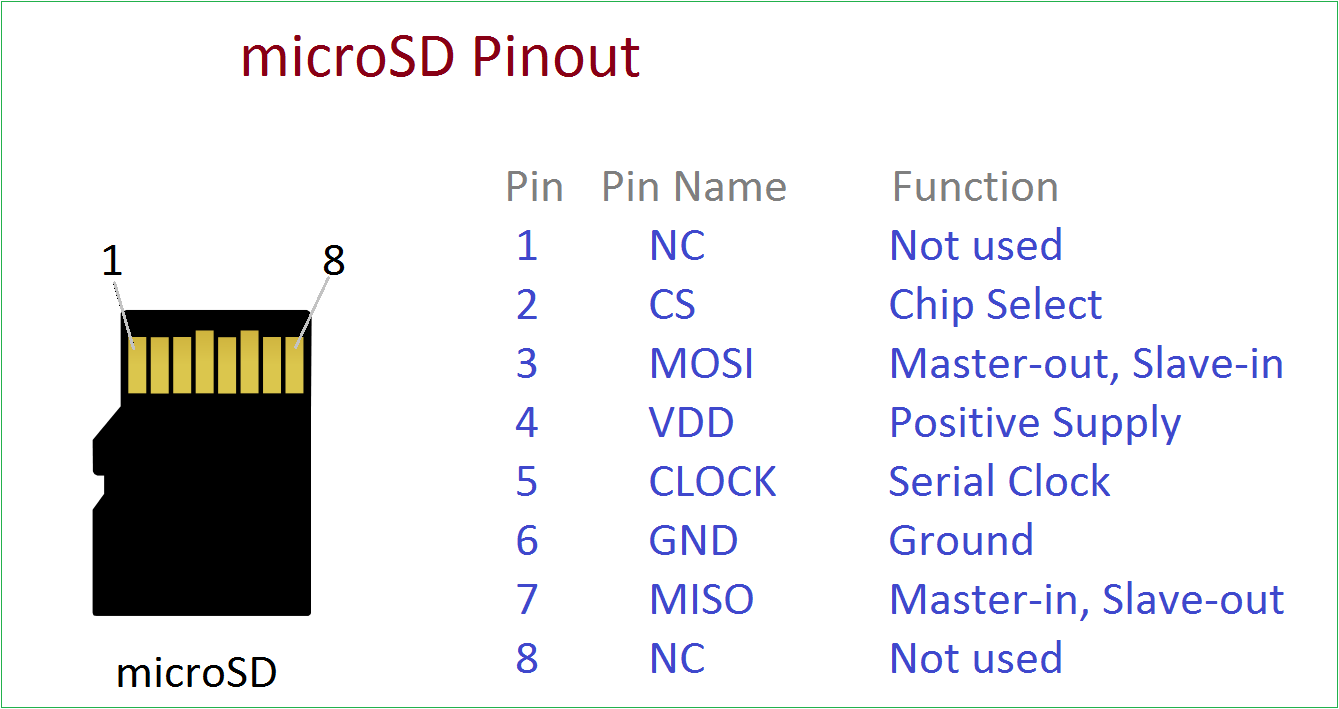
\includegraphics[width=0.55\textwidth]{graphics/micro-sd-pinout}
	\caption{Pinout des mikroSD-Sockels.}
	\label{fig:micro_sd_pinout}
\end{figure}

\todo{cite: https://www.ecosia.org/images?q=mikroSD+pinout\#id=F8E296D6DF751D79D199FC7711B8A9D178456B6F}

Als Dateisystem wird FAT32 verwendet. FAT32 steht für File Allocation Table mit 32Bit Datenbreite. Es ist ein von Micosoft entwickeltes System, dessen Wurzeln bis ins Jahr 1977 zurückreichen und heute noch der Industriestandard unter den Dateisystemen ist.

\todo{cite: https://www.ionos.de/digitalguide/server/knowhow/fat32/}

Der Speicherbereich einer FAT32-formatierten Partition besteht aus fünf Bereichen.
\begin{enumerate}
\item Master Boot Record (LBA Sektor 0 des Laufwerks)
\item Volume Boot Record, Partition Boot Sektor (LBA Sektor 0 der Partition)
\item File Allocation Table (i.d.R 2 mal hintereinander vorhanden, direkt nach dem PBR)
\item Directory Table (mit den Ordner und Fileeinträgen)
\item Datenbereich (Fileinhalt)
\end{enumerate}

\todo{cite: https://docplayer.org/78333139-Aufbau-des-fat32-dateisystems.html}

Im \textbf{Master Boot Record} ist ein Startprogramm vorhanden, welches für BIOS baseierte Computer geschrieben wurde.
Darin enthalten sind der Boot-Code in Assembler, Fehlermeldungen je nach Landessprache, Darstellungen der Fehlermeldungen, die Disk Signature, für die Organisation des Laufwerks wichtige Partitionstabelle und die Signature ID oder auch Magic Number 0x55 0xAA. Hier wird die aktive Partition ausgewählt und der Boot Sektor geladen. Da nicht über die SD-Karte gebootet wird, besteht dieser Teil nur aus Gründen der Kompatibilität.

\todo{cite: https://www.german-sales.com/datenstruktur.htm}

\todo{cite: https://docplayer.org/78333139-Aufbau-des-fat32-dateisystems.html}

Im \textbf{Volume Boot Record} befinden sich 3 Sektoren. Der erste Sektor enthält einen Sprungbefehl und einen ''tu nichts'' Befehl (''nop''), den Systemname (OEM ID), den BIOS Parameter Block, den Boot Code, der Bootloader File Name, Fehlermeldungen, Darstellung der Fehlermeldungen und ebenfalls die Magic Number 0x55 0xAA. Der zweite Sektor enthält den Anfang des erweiterten Volume Boot Records eines FAT32 Systems, den Anfang der Daten und das nächste verfügbare Cluster sowie die Magic Number. Hier kann kalkuliert werden, wieviel freier Speicher noch verfügbar ist. Der dritte Sektor ist eine Erweiterung des ersten Sektors, falls der Speicher für den Bootcode nicht ausreicht. Unter FAT32 wird für die drei Sektoren eine Sicherheitskopie abgelegt, welche zur Wiederherstellung des Volume Boot Records dient.

Im \textbf{File Allocation Table} wird organisiert, welche Cluster auf der Partition belegt oder frei sind und wo die Folgecluster eines Files sind. Die Clustergrösse kann selbst bestimmt werden und beträgt bei SD-Karten mit kleinen Dateien optimalerweise 512Bytes. Dies ist die minimale Grösse, da ein Cluster aus mehreren Sektoren besteht und ein Sektor 512 Bytes gross ist. Für die Cocktailmaschine weden pro File ca. 100 Bytes verwendet, wodurch pro File ca. 412 Bytes unnutzbar werden. Der Nachteil ist, dass die FAT so grösser wird und grosse Dateien mehr zerstückelt werden. Die Cluster sind fortlaufend nummeriert, wobei sich die Nummerierung in der FAT immer auf den Ort innerhalb der FAT bezieht, nicht auf den realen Ort auf der Partition. Ist ein File grösser als 512 Bytes, so ergibt sich eine Clusterkette, welche einen Verweis auf das nächste Cluster enthält und ein Verweis, falls die Kette zu ende ist. Jeder Eintrag der FAT ist 32 Bit lang (4 x 8 Bytes = 4 Doppelwörter). Ein Cluster kann z.B den Wert 0x0E 00 00 00 haben, wobei der Verweis 0E auf das nächste Cluster zeigt. Ein Endcluster ist mit dem Doppelwort 0xFF FF FF 0F gekennzeichnet. Ist eine Datei Fragmentiert, ist die Nummerierung nicht fortlaufend, sonder spring hin und her. Konklusion: Die Werte innerhalb des FAT zeigen an, ''wo sich relativ gesehen die Daten eines Files auf der Partition finden lassen. Dabei sind die Werte entweder das Zeichen für ein Clusterende oder sie zeigen auf den nächsten Cluster der Clusterkette innerhalb der FAT'' \todo{cite: https://docplayer.org/78333139-Aufbau-des-fat32-dateisystems.html}. Um jedoch das Anfangscluster auf der Partition finden zu können, muss das Directory Table angeschaut werden.

\newpage

Im \textbf{Directory Table} sind alle Files und alle Ordner der Partition beschrieben. Der Startsektor errechnet sich aus der letzten FAT und der Grösse der FAT (Addition). In diesem Bereich befindet sich das Root Directory, oder auch Wurzelverzeichnis genannt. Es hat eine hiararchische Baumstruktur, was bedeutet, dass ''das Wurzelverzeichnis das oberste mögliche Verzeichnis ist unter dem sich weitere Verzeichnisse befinden können'' \todo{cite: https://docplayer.org/78333139-Aufbau-des-fat32-dateisystems.html}. Bis auf das Wurzelverzeichnis haben alle anderen Verzeichnisse ein einziges Elternverzeichnis, können aber mehrere Unterverzeichnisse haben.

\todo{cite: http://www.informatik.uni-ulm.de/ni/Lehre/WS01/TI2/folienmb/fat32slide.pdf}

Der Name des Files ist in der Regel 8 Bytes lang, worauf 3 Bytes folgen für die Bezeichnung der Fileart (z.B .txt). Ein Byte steht für die Volume ID, welche Attribute das File oder der Ordner hat. Hier befinden sich der Zeitstempel des Files, das Datum des letzten Zugriffs und das Datum der letzten Änderung des Files. Vier Bytes enthalten das Startcluster des Files oder des Ordners, vier weitere Bytes enthalten die Grösse des Files. Die restlichen Bytes sind mit 0x00 beschrieben. Um den tatsächlichen Startsektor auf der SD-Karte zu finden, wird eine Umrechnungsformel benötigt. Diese und ein Beispiel wie die File-Organisation aussieht, kann dem File ''Aufbau des FAT32 Dateisystems'' entnommen werden.

\todo{cite: https://docplayer.org/78333139-Aufbau-des-fat32-dateisystems.html}

Die Ordner sind auf die selbe Weise organisiert, bis auf die Ausnahme, dass in FAT32 keine Grössenangaben für Ordner gemacht wird. Die Bytes werden deswegen mit dem Wert 0x00 beschrieben.

Für die Cocktailmaschine wird deswegen eine Library benötigt, welche die FAT32-Commands implementiert und geichzeitig die Operationen auf der SD-Karte handelt. So ist die SD-Karte auch am Computer editierbar und die Befehlsliste reduziert sich auf readFile, writeFile und deleteFile.